\section{Support in Score-P and Vampir}

The following sections present the level of support for modern C++ by Score-P and Vampir. Most features are already supported by both tools; the focus therefore lies on missing capabilities. This is achieved by implementing several small example programs that make use of these features. The source code of these examples can be found in Appendix \ref{app:scorep}. The code is compiled with GCC 6.2.1, using the compiler plugin from Score-P 3.0. The results are examined using Vampir 9.0.

\subsection{Concurrency}\label{scorep:conc}

In this section the various concurrency constructs introduced in C++11 is discussed.

\subsubsection{\texttt{std::async}}\label{scorep:conc:async}

As mentioned in Section \ref{modern:queue:futures} \texttt{std::async} is a high-level construct to asynchronously run tasks. The underlying management of threads is not exposed to the library user; instead, it is guaranteed that the result is returned upon a call to \texttt{std::future::get} (\texttt{std::async} returns a \texttt{std::future}). This may lead to blocking on the caller's side if the asynchronous task has not been completed yet. This potential bottleneck makes any application using \texttt{std::async} a natural target for performance analysis, even more so as its default behaviour with regard to thread spawning is implementation specific.

There are three test cases in this document: One for the default behaviour (Appendix \ref{app:scorep_conc_async_default}), another for explicit asynchronous evaluation (Appendix \ref{app:scorep_conc_async_async}) and a third for explicit lazy evaluation (Appendix \ref{app:scorep_conc_async_lazy}).

The first two test cases fail with the following error message (when compiled with GCC 6.2.1):

\begin{verbatim}
$ SCOREP_ENABLE_TRACING=1 ./future_default                                      
[Score-P] src/measurement/thread/create_wait/scorep_thread_create_wait
          _pthread.c:84: Fatal: Bug 'tpd == 0': Invalid Pthread thread
          specific data object. Please ensure that all pthread_create
          calls are instrumented.
[Score-P] Please report this to support@score-p.org. Thank you.
[Score-P] Try also to preserve any generated core dumps.
[Score-P] src/measurement/thread/create_wait/scorep_thread_create_wait
          _pthread.c:84: Fatal: Bug 'tpd == 0': Invalid Pthread thread
          specific data object. Please ensure that all pthread_create
          calls are instrumented.[1]    8405 abort (core dumped)
\end{verbatim}

\noindent Unfortunately, imitating \texttt{std::async}'s behaviour with the Pthread library for the sake of this document is impossible as the thread management behind the call is implementation-defined: the library may spawn operating system specific threads internally, rely on a thread pool or do something entirely different.

The lazy evaluation test case executes successfully; however, because the code in question is not executed in a separate thread the inspection of Score-P's trace file shows nothing noteworthy.

\subsubsection{\texttt{std::thread}}\label{scorep:conc:thread}

When compared to \texttt{std::async}, \texttt{std::thread} follows a more ``low level'' approach as thread execution is now entirely in the hands of the user. Naturally C++11 threads are profiling targets, too.

There are two test cases for \texttt{std::thread}: the first spawns a thread and joins it afterwards (Appendix \ref{app:conc_thread_join}), the second spawns a thread and detaches it, making it unjoinable (Appendix \ref{app:conc_thread_detach}).

Both test cases fail to execute and produce the same error message already known from Section \ref{scorep:conc:async}. Because \texttt{std::thread} simply wraps a Pthread (at least in libstdc++) its behaviour can be emulated. Figures \ref{scorep:conc:pthread_join_timeline} and \ref{scorep:conc:pthread_detach_timeline} are created by profiling such an emulation.

Figure \ref{scorep:conc:pthread_join_timeline} shows the creation of a thread by the master thread (the first blue block). Afterwards the master thread tries to join the new thread (the second blue block). This call blocks the master thread as indicated by the black lines connected to the thread execution (lower green block). The master thread can only resume once the spawned thread has completed its work, indicated by the second black line.

Figure \ref{scorep:conc:pthread_detach_timeline} show the creation of a thread by the master thread (blue block). This thread is then detached, meaning it is left in an unjoinable state. The master thread continues its own work (upper green block) while the detached thread runs in parallel (lower green block).

\begin{figure}[htbp]
	\begin{center}
		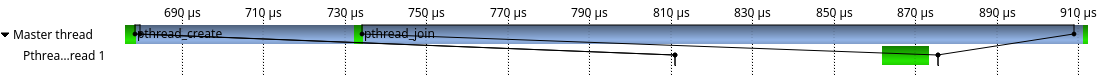
\includegraphics[width=0.9\textwidth]{img/scorep_pthread_join_timeline.png}
		\caption{Emulated master timeline for a joined \texttt{std::thread}}
		\label{scorep:conc:pthread_join_timeline}
	\end{center}
\end{figure}

\begin{figure}[htbp]
	\begin{center}
		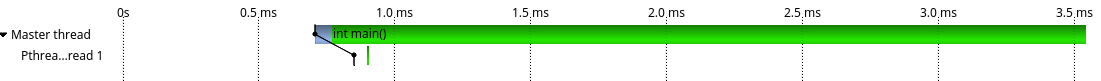
\includegraphics[width=0.9\textwidth]{img/scorep_pthread_detach_timeline.png}
		\caption{Emulated master timeline for a detached \texttt{std::thread}}
		\label{scorep:conc:pthread_detach_timeline}
	\end{center}
\end{figure}

\subsubsection{Summary}

At the time of writing, Score-P's support for C++11 multithreading is nonexistent as the error messages from Section \ref{scorep:conc:async} and Section \ref{scorep:conc:thread} show. The likely cause for these errors lies in the internals of the GNU C++ compiler's standard library because the threading support library is compiled into the shared library object. Score-P is unable to instrument this already compiled code and crashes upon execution once it encounters an unknown thread.

The solution for this problem would be a more graceful handling of ``unknown threads'': Instead of crashing, Score-P should simply register them on the fly. As of September 2016 there is a new Score-P development branch adressing this issue.

The visualisation in Vampir should offer the same look and feel as the visualisation of Pthreads. That means:

\begin{itemize}
\item Vampir should draw a line between the call to \texttt{std::future::get} or \texttt{std::future::wait} and the actual end of the related function and from there to the end of the call. Like a Pthread thread the asynchronous task should be visible as a separate block on the master timeline. If the task was launched with the \texttt{std::launch::deferred} parameter no visualisation is needed as it shared the same thread of execution with its caller.
\item When using \texttt{std::thread} the Pthread interface can be widely reused. It should not show the underlying native threads but the calls to the \texttt{std::thread} interface, e.g. \texttt{std::thread::join} instead of \texttt{pthread\_join}. The visualisation of thread interdependencies should be identical, i.e. black lines from the call to the thread and back to the end of the call.
\end{itemize}

\subsection{Synchronisation}

With the introduction of the thread support library synchronisation primitives were added to the standard library as well. Because such primitives are able to block thread execution, profiling their behaviour is especially interesting in a HPC performance analysis context. In this section the mutual exclusion constructs (\texttt{std::mutex}) and condition variables (\texttt{std::condition\_variable}) are evaluated. Due to the problems shown in Section \ref{scorep:conc} the spawned threads in the testcases are emulated by using the Pthread library.

\subsubsection{\texttt{std::mutex}}\label{scorep:sync:mutex}

\texttt{std::mutex} and its more specialised siblings \texttt{std::timed\_mutex}, \texttt{std::recursive\_mutex} and \texttt{std::recursive\_timed\_mutex} provide simple mechanisms for mutual exclusion between threads, namely locking and unlocking. However, directly accessing these mechanisms is not exception-safe which is why they are usually managed by \texttt{std::unique\_lock} or \texttt{std::lock\_guard}. Relying on \gls{raii} these primitives will automatically unlock the managed \texttt{std::mutex} once they leave their scope.

The test case (see Appendix \ref{app:scorep_sync_mutex}) utilizes them for synchronisation between two threads instead of locking the \texttt{std::mutex} manually. Upon execution the test case itself works as expected: threads are spawned and \texttt{std::mutex} blocks one of them while being locked by the other.

Score-P on the other hand is not able to fully parse the instruction flow correctly: instead of instrumenting the calls to the standard library facilities it detects and instruments the underlying Pthread mechanisms utilised by the library implementation, shown by Figures \ref{scorep:sync_pthread_mutex_timeline} and \ref{scorep:sync_pthread_mutex_summary}. This can be explained by the compiler's inlining of the \gls{stl} functions which prevents Score-P from instrumenting the actual function call. The black lines in Figure \ref{scorep:sync_pthread_mutex_timeline} connecting the threads are known from Section \ref{scorep:conc:thread} and indicate thread joining. The red block seen in one thread symbolises a blocking call to the mutex's locking routine.

\begin{figure}[htbp]
	\begin{center}
		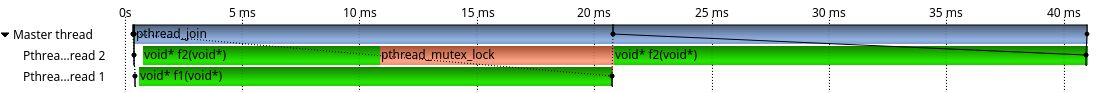
\includegraphics[width=0.9\textwidth]{img/scorep_pthread_mutex_timeline.png}
		\caption{Master timeline for thread synchronisation with \texttt{std::mutex}}
		\label{scorep:sync_pthread_mutex_timeline}
	\end{center}
\end{figure}

\begin{figure}[htbp]
	\begin{center}
		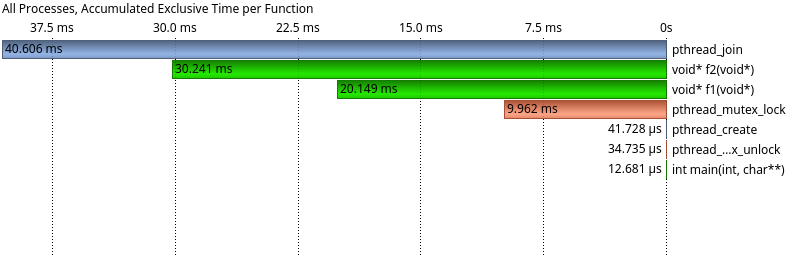
\includegraphics[width=0.9\textwidth]{img/scorep_pthread_mutex_summary.png}
		\caption{Function summary for thread synchronisation with \texttt{std::mutex}}
		\label{scorep:sync_pthread_mutex_summary}
	\end{center}
\end{figure}

\subsubsection{\texttt{std::condition\_variable}}\label{scorep:sync:cv}

\texttt{std::condition\_variable} is the other synchronisation primitive added to the standard library with C++11, allowing threads to communicate with each other. A \texttt{std::condition\_variable} is always associated with a \texttt{std::mutex} but offers more fine-grained control via its notification mechanisms -- a thread can either wake up one other waiting thread or all of them.

The test case (see Appendix \ref{app:scorep_sync_cv}) spawns four threads, of which three are waiting for the fourth to signal them. Once they receive the notification they execute their instructions in parallel.

Like the simpler \texttt{std::mutex} test case (see Section \ref{scorep:sync:mutex}) this program executes successfully and suffers from the same problems with inlining (see Figures \ref{scorep:sync_pthread_cv_timeline} and \ref{scorep:sync_pthread_cv_summary}). Again, the red blocks indicate mutex locking or unlocking; the lines connecting the individual threads with the master thread represent thread joining operations.

\begin{figure}[htbp]
	\begin{center}
		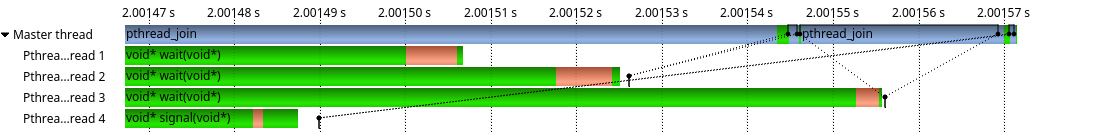
\includegraphics[width=0.9\textwidth]{img/scorep_pthread_cv_timeline.png}
		\caption{Master timeline for thread synchronisation with \texttt{std::condition\_variable}}
		\label{scorep:sync_pthread_cv_timeline}
	\end{center}
\end{figure}

\begin{figure}[htbp]
	\begin{center}
		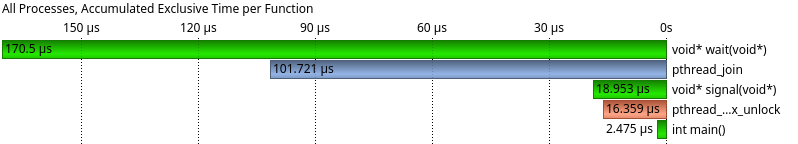
\includegraphics[width=0.9\textwidth]{img/scorep_pthread_cv_summary.png}
		\caption{Function summary for thread synchronisation with \texttt{std::condition\_variable}}
		\label{scorep:sync_pthread_cv_summary}
	\end{center}
\end{figure}

\subsubsection{Summary}

While Score-P and Vampir generally support the instrumentation of mutex operations they fail to do this correctly for the \gls{stl} because of inlining. In order to change this, Score-P would need a mechanism to instrument the \gls{stl}'s interface without automatically instrumenting all the inlined implementation details behind the interface.

The visual representation by Vampir could be adapted to work with the \gls{stl} interface. Drawing connection lines between related mutex locking and unlocking operations would improve the user experience even further; these are not needed if threads are not actually waiting on each other despite using the same mutex (i.e. thread 1 unlocks the mutex before thread 2 tries to lock it -- thread 2 is not blocked in this case and a connecting line does not make sense).

\subsection{File I/O}

While file I/O is not a new concept and has not changed with C++11 its performance penalties are still an important issue to consider in an HPC context. This section represents the evaluation of file I/O using C++ file streams as well as the C API.

\subsubsection{C++ Filestreams}\label{scorep:fstream}

The first test case (see Appendix \ref{app:scorep_fstream}) generates a \texttt{std::vector} with random integer values and writes them to a file. The file itself is created and modified by a \texttt{std::ofstream} opened in binary mode. It is then closed and opened again by a \texttt{std::ifstream} which then proceeds to read its contents into another \texttt{std::vector}.

At the time of writing all file operations using C++ streams are ignored by Score-P and Vampir.

\subsubsection{C-style I/O}\label{scorep:c_io}

The result of Section \ref{scorep:fstream} may lead to the conclusion that the file operations are inlined by the compiler and thus not visible to Score-P. The second test case implements the functionality from Section \ref{scorep:fstream} using the API inherited from the C standard library (see Appendix \ref{app:scorep_c_io}).

Again, Score-P and Vampir ignore all file operations. This shows that the issue is not related to inlining but to Score-P not instrumenting standard library and/or system calls.

\subsubsection{Summary}

As of September 2016 Score-P does not support the instrumentation of file I/O. There is, however, a development branch targeting these issues for the C API, representing file operations as horizontal black arrows on the master timeline. From a usability perspective it might be more intuitive to represent them as black blocks (similar to Pthread library calls) instead of arrows.

The visualisation of C++ file I/O should look similar to the proposed C API visualisation; a call to \texttt{std::fstream::write} is usually interchangeable with a call to \texttt{std::fwrite} since both operate on the level of individual bytes.

\subsection{Lambdas}

Lambda functions are especially useful when used in conjunction with the functions found in the header file \texttt{<algorithm>}. This naturally makes them a profiling target. Usually they are inlined because of their small code size which renders them invisible for Score-P.

In cases where inlining does not occur Score-P faces two minor naming issues. The first issue can be reproduced by the following code:

\begin{minted}[fontsize=\small]{c++}
auto my_lambda = [](int i) { //... };
\end{minted}

\noindent If this code does not get inlined for whatever reason\footnote{Unfortunately, this behaviour was not reliably reproducible which is why there is no test case in the appendix. The lambda's symbols are present in the executable but they are still not visible to Score-P.} Score-P will show the following name:

\begin{minted}[fontsize=\small]{c++}
main::{lambda(int)#2}::operator()(int) const
\end{minted}

\noindent This naming is very unintuitive and does not help the user in quickly identifying hotspots. The situation becomes worse when using an \texttt{auto} parameter, a feature introduced in C++14:

\begin{minted}[fontsize=\small]{c++}
auto my_lambda = [](auto i) { // ... };

_ZZ4mainENKUlTE_clIiEEDaS_ // called with "int" parameter
_ZZ4mainENKUlTE_clIdEEDaS_ // called with "double" parameter
\end{minted}

\noindent Both issues are not Score-P's fault but originate in GCC's naming and mangling scheme. To work around this, Score-P would need to implement a custom naming mechanism which works around the one imposed by GCC. The easier alternative for the second issue is to wait for a GCC bugfix which improves generic lambda name mangling.